\chapter{\textit{Grasp}について}
\label{graspについて}

\section{概要}
第\ref{about_grasper}章では、作品概要と、そこに至るまでのプロトタイピングの分析を通して、作品形態について説明した。

第\ref{graspについて}章では、本研究が提示するコンセプトである\textit{grasp}について詳細に説明する。その上で、Felsの分類との関係性と、この概念を用いることから修士作品の体験についてのねらいを説明する。

\section{\textit{grasp}の定義}
\label{grasp_difinition}
\textit{grasp}について、本研究では次のように定義する。

\begin{quote}
  \textbf{人と対象との関係の中で、人が対象の中に注意や目的意識を抱きながら、意識的に試行する期間}
\end{quote}

graspは「把握」を意味する動詞でもあるが、ここで「動作」ではなく「期間」とした。その理由は、「意識的に試行する」とき、同時にその結果を受けて気づきを得たり、その気づきをもとに新たな関心を抱くといった、単に自分が行為しているだけではなく、対象から影響を受けながら次の行為が決まってくるようなフィードバックループの構造があると考えるためである。「grasp=把握」という言葉についても、単に「ものを掴む」という意味だけでなく、「理解」の意味があることは、対象について一方向に働きかけているのではない様子が現れているのではないだろうか。

\textit{grasp}とは例えば、ギターの習得過程において、弾きこなしたいフレーズを定め、それを達成するまでに試行錯誤をし、達成できるようになるまでの期間である。熟達した状態では、熟達する前とは違う視座でものごとを捉えられるようになり、また違う対象に注意が向くようになると、ギターと人との間に別の\textit{grasp}が芽生える。
またあるいは、\textit{grasp}の過程で、対象と向き合い続ける過程の中でその解像度が高まり、当初目指していたこととは違うことに興味を抱く(セレンディピティ)ことでも、別の\textit{grasp}が芽生える。

ここまで具体例を通してみてきたように、\textit{grasp}は、ギターと人との関係において一度だけ生じるのではなく、注目する対象が定まれば何度でも生じる。
% ここで、\textit{grasp}は人と対象の関係の中で、人が注意を向ける「対象」ごとに別の\textit{grasp}があると言えそうだが、注意を向けている「対象」がなんであるか、断言できなかったり、本人も判然としないこともある。そのため、

\section{Felsの議論との関係性}
ここでは\textit{grasp}が、FelsのEmbodimentとどう関係するのかについて説明する。
先の節\ref{grasp_difinition}に挙げたように、人は\textit{grasp}を通して、あるいはその過程で、対象から影響を受けながら次の試行が形作られていく。この時の「試行」には、挙動を確かめるような動作、すなわちFelsの「Response」もあれば、試行を通して得られた結果をもとに、何かに考えを巡らす「Contemplation」も含まれる。こうした試行の積み重なりから、人と対象のあいだに「Control」や「Belonging」の関係、すなわちFelsの意味でのEmbodimentが生じるのではないか。

つまりこの概念は、折り合いをつけていくまでの「間」に行われていることについて語ることを可能にするものである。\textit{grasp}の様相を捉えることで、現状からEmbodimentが達成されるまでのあいだに欠けているものが何であるかを語る術を得られるのではないか、と考える。

\section{\textit{grasp}を踏まえたIntimacyが起こるまでの過程についての仮説}
\textit{grasp}が、本研究の関心である「対象からの影響も受けつつ(Belonging)、相互の折り合いをつけながら生まれる一体感(Intimacy)が起こる」までの過程に必要ではないか、と考える。

そしてそのためには、注意を向ける対象や目的意識を抱く対象が変わりながらも\textit{grasp}が継続していく体験が良いのか、それとも注意を向ける対象は変わらず、1つのものに対する目的意識が長く継続し、\textit{grasp}も長い体験が良いのか。このいずれであるかが判別することができれば、より詳細にこの体験を説明することができると考えた。

\section{\textit{grasp}を用いた《Grasp(er)》の説明}
本作品を\textit{grasp}の観点から、どのような関係が芽生えることがそのねらいとしてあるかについて、それぞれの作品について説明する。

\subsection*{Familiar / Strange(執筆中)}
後に出てくる「Relation」に比べると、\textit{grasp}の時間は短く、複雑度も低いため、この過程で体験者独自の試行が行われることは多くはない。しかし学内での展示に際して、徐々に変換が複雑になる中で、「ある形を作ってみようとする」ことや「途中から追いつけなくなった法則性を確かめる」ように手指を動かす方がいた。

\subsection*{Relation(執筆中)}
ボールという直接的に制御することができない対象とのあいだでのGraspを経験するので、\textit{grasp}の時間は長い。その過程で「左右に転がしてみる」、「投げ上げる」、「受け止める」といったことを試行する、前の作品よりも注意の向く対象が多い作品である。そして、このとき「自発的に芽生えた目的意識」こそが、制作者の意図を超えたものであると考える。

% \textit{grasp}には二つの性質がある。一つは、時間幅が注意を向けている対象によって、長い場合と短い場合があることである。目的意識が芽生えてからスムーズに操作できるようになる場合、'reach'から'manipulate'が近く、\textit{grasp}は短い、すなわち直感的で使いやすいものとして経験される。その一方、目的意識が芽生えてから試行錯誤を伴い、習熟に長い期間を要する場合、\textit{grasp}は長く、もどかしさを経験し、操れるようになった時に達成感を経験する。\\

% 二つ目に、\textit{grasp}の過程で他のことに対する意識が次々と芽生えることがある。具体的には「やってみるまでわからない」といった経験や、物事に対する解像度が高まる中で、当初とは異なる意識が芽生える状況に相当する。\\

% このコンセプトを展開し、「試行錯誤の余地」を設計することを目指したのが、修士作品《Grasp(er)》である。この作品では、\textit{grasp}を経験する中で、個人による創造的な活動が生まれ、\textit{grasp}という動作を行っているのではなく、そこに'er'の接尾辞がついた'Grasper'であると名付けた。

\section{プロトタイピング}
本作品の形態に至るまでに、総計60パターンのプロトタイプ制作を行なった。プロトタイピングにおける目的を時系列で3段階に大別すると、「テーマの着想」、「変換表現によって錯覚する「手触り」についての発散」、そして「表現の収束」である。「テーマの着想」に至るまでのプロトタイピングについては、前節\ref{prototyping_concept_making}にて説明した。ここでは、後の2つについて説明する。

\subsection{変換表現についての探索(執筆中)}
「手指の変換表現」の中でも、単に形を考えるだけでなく、どの動きをその形に当てはめるか、そしてどの時間の動きを用いるか等、さまざまな変換方法が考えられる。この段階では先入観によって絞り込むことがないよう、このような探索空間の中で思いつく限り実装し、実際に体験することを通して判断するという姿勢でプロトタイピングをおこなった。以下では、行ったプロトタイピングについて「形状」、「構造」、「時間操作」の観点から分類し、それぞれの概要を説明する。その上で、これらのプロトタイピングを通してどのような知見を得て、次の探索へつながったのかについての説明を「振り返り」としてこの節の最後に述べる。

\subsection*{形状}
形状については、指を動きの最小単位として、指ごとに独立したバリエーション、指同士を直列に繋ぎ合わせたバージョン、円形に繋ぎ合わせたバージョンなどを作成した。また、単位である指をどのように表現するかについては、「円形」、「くの字」、「ひょうたん型」などのバリエーションで表現を試みた。
\begin{figure}[H]
  \centering
  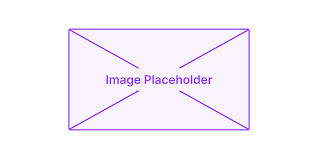
\includegraphics[width=15cm]{img/placeholder.png}
  \caption{ユニットのバリエーション}
  \label{fig:unit_valiation}
\end{figure}
\subsection*{マッピングの方法}
マッピングについては、1つの動きを複製して、1つの動きを複数のパーツの動きへと波及させるバリエーションなどを作成した。図\ref{fig:networked_finger}に示すプロトタイプでは、指先をクリックすると5本ある指のうちのいずれかの動きを追従する指が、指先に追加されるものである。どの指が付け加わるかはランダムで、指が新しく追加されるたびに、それがどの指の運動であるかを同定するには、一本一本指を動かして、どこがその指に対応しているのかについて同定する必要がある。
\begin{figure}[H]
  \centering
  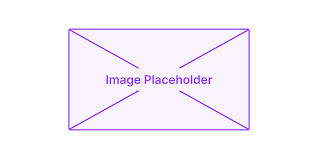
\includegraphics[width=15cm]{img/placeholder.png}
  \caption{Networked Finger}
  \label{fig:networked_finger}
\end{figure}

またそのほかに、図\ref{fig:fractal_finger}に示すプロトタイプでは、親指の先に人差し指の動きが複数分岐し、さらに人差し指の先から中指の動きが複数分岐して配置される、といったフラクタル構造で指の動きを配置したパターンを制作した。このように、配置を変えるだけでなく1つの指の動きに対して対応して動く部分を多数にするなどのバリエーションを検討した。

\begin{figure}[H]
  \centering
  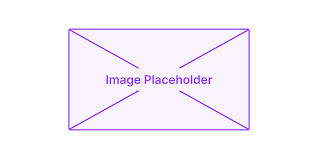
\includegraphics[width=15cm]{img/placeholder.png}
  \caption{Fractal Finger}
  \label{fig:fractal_finger}
\end{figure}
\subsection*{時間操作}
最新の自分の動きだけを表示するのではなく、過去の動きも表示するプロトタイプにも取り組んだ。図\ref{fig:prototype_delay}に示すプロトタイプでは、5本の指の動きが等間隔に並べられているが、それぞれの指は、鉛直上向きの角度に現在の指の動き、そこから時計回りに、順次過去の指の動きが並べられている\footnote{https://interaction005-moe5dbh11-k1105.vercel.app/}。

このプロトタイプでは、指先を小さく動かすと、その動きが時計回りに伝播していくようすが見て取れる。これは例えばゼリー状の物体を触れた時のような、衝撃が物体全体へと伝播していくようすに見立てられるため、柔らかいオブジェクトに触れているときのような身体感覚を錯覚することがある。

\subsection*{振り返り}

\begin{figure}[H]
  \centering
  
\includegraphics[width=15cm]{img/past_time.png}
  \caption{過去の動きを用いた例}
  \label{fig:prototype_delay}
\end{figure}
\subsection{表現の収束(執筆中)}
ここまで行なってきたプロトタイプから方向性を絞り、ブラッシュアップした。
\subsection*{動かしている感覚が強い表現}
1つ目の観点として、手指の微細かつ複雑な動きをもって、緻密な制御をしているという感覚が引き出される表現へと絞り込んでいくことにした。

その上で注目したのは、「関節を折り曲げる動き」に対する共感性である。
人間の手指は

その一方で、円の半径に関節の動きをマッピングさせるような表現については、縮んだり、膨らんだりする動きには共感しづらい。微細な運動が増幅される「気持ちよさ」があるが、この気持ちよさは身体動作との連動によってもたらされる気持ちよさではなく、動作に対するフィードバックに対する快、すなわちFelsのいう「Response」による快が強い。

また、1つの動きを複製して円形に配置したり、フラクタル的に配置するパターンを排除した。これについては、グラフィックデザイナーの女性が体験した際「構造としては緻密であるのに、動きは単純であるように感じる」と意見した。その理由として彼女は、「対称性が前面に出ているため、シンボルとしての印象を強く感じてしまう」「意識していないところも同時に動いている感覚があるため、自分の動きだと思えない」からではないかと推測した。

\subsection*{注意の対象による作品の分割}
一方で、プロトタイピングを通して同定した変換表現を通して生じた異なる身体像に対する共感覚のようなものは、変換された手を用いた作業に移行した瞬間に、注意が向きづらくなるといった課題が起こった。そこで、最終的な作品としてはその2つを分けて構成した。

\subsection*{モーフィング}
「身体の変容」を扱っている本作では、取得されたキーポイントの位置を大きく変更させることで、「意図的にIntimacyを下げる」操作を行なっている。しかし「下がった」という事実を体験者が認識するために、もとの手が鏡合わせのように出力されている状態から、徐々に形を変えていくようすを連続的に示すモーフィングを実装している。

過去に展示していたバージョンではモーフィングを示さず、手指が認識されたとたんに全く違う手指が提示される作品形態であった。しかし、この形態で展示した場合、画面の中の手指と自身の関係性について、全く異なる生命体のようなものを、操り人形のように自分の手指の指令によって動かす、といったような関係性として認識されることがあった。また、全く見慣れない形なので、「手指を細かく動かせる」といった、作品がもつ可能性に気づけない場合があることがわかった。そこで、このモーフィングを実装することで、白い点が関節を表していること、そして手指の運動を細かくトラッキングしていることを事前に伝え、それが形を変えた姿として画面の前に提示されていることを示す形態を採用することになった。
そうすることで、画面に出力されているグラフィックと身体との関係性は別々の存在ではなく、自分の身体であったことが明示される。

\subsection{展示形態の設計}
展示形態について、時系列順に過去2つのバージョンについて説明し、その流れから最終的な展示形態の根拠を示す。

\textbf{初期:カメラを画面前に配置した状態}\\
最初期は、体験装置について下図\ref{fig:kyotai_ver0}のように、モデルトラッキングを行っているカメラを直接画面の前に配置していた。
\begin{figure}[H]
  \centering
  \includegraphics[width=15cm]{img/kyotai_ver0.jpg}
  \caption{初期:カメラを画面前に配置した状態}
  \label{fig:kyotai_ver0}
\end{figure}

プロトタイピングの段階でもあったため最低限の構成としていたが、この構成には次のような問題があった。
\begin{quote}
  \begin{itemize}
    \item カメラのトラッキング精度が環境光の影響を受けて変動してしまう
    \item 体験者ではない周囲の人の手指を間違ってトラッキングしてしまう
    \item 手指の形がそのまま出力されるわけではないので、トラッキングの範囲がわからず、腕を大きく振ったり、手指がトラッキングできない範囲で動かしてしまう
  \end{itemize}
\end{quote}

このため、制作者が指示をすることなく自由に体験してもらうことを意図していた展示であっても、体験方法がわからなかったり、後方で見守る人の手を誤ってトラッキングしてしまうといった問題が起き、有効なフィードバックを得ることができなかった。

\textbf{中期:専用筐体を用いて手首を固定した状態}\\
こうした課題を踏まえて、次に専用筐体を制作し、穴に手を入れる形式について試した(図\ref{fig:kyotai_ver1})。

\begin{figure}[H]
  \centering
  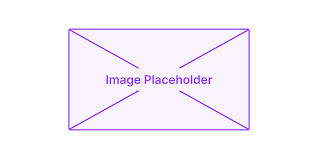
\includegraphics[width=15cm]{img/placeholder.png}
  \caption{中期:専用筐体を使用してカメラを隠蔽した状態}
  \label{fig:kyotai_ver1}
\end{figure}

この形式では、カメラの画角に映り込むのは筐体の内部と体験者の手のみであるため、環境光の影響や周囲の人の影響を受けずに体験してもらうことが可能となった。また、穴によって手首の位置が固定されるため、腕を大きく振ることが構造上不可能となり、比較的身体動作の幅が抑えられた。

ただし、この形式は単に上記の問題を解決したというだけではなく、指先の動きが見えなくなったこと、画面に対する指先の位置関係についてを変更するものであった。

画面に対する手指の位置関係については、本作品では手指の形状が、もとの形とは全く関係のない構造へと変化するため、作品体験には大きな影響はないと判断した。手指の動きが見えなくなったことについては、画面の中の手指は体験時、自身の身体に代わる存在であるから、同時に視認できない今の形態の方がむしろ、より適した構成であると判断した。

しかしその一方で、手首の動きを固定してしまったことは、身体の動きを過剰に限定してしまう結果となった。身体の動きを限定してしまうと、何か特定の動作を求められているような説明的な構成になってしまう。そのため筐体としては、より簡素な構成が好ましいと判断した。


\textbf{作品展示:専用筐体を用いて手首を固定せず指先を自由にした状態}\\
そこで最終的には、図\ref{fig:kyotai_ver2}のような、トラッキングの範囲を暗示しながら、手首を固定しない方式に変更した。また、トラッキングに用いるカメラを、視野角150°の広角カメラ(Sanwa Supply CMS-V43BK-3)に変更し、大きく手指を動かしてもトラッキングの外れることの少ないものへと変更した。

\begin{figure}[H]
  \centering
  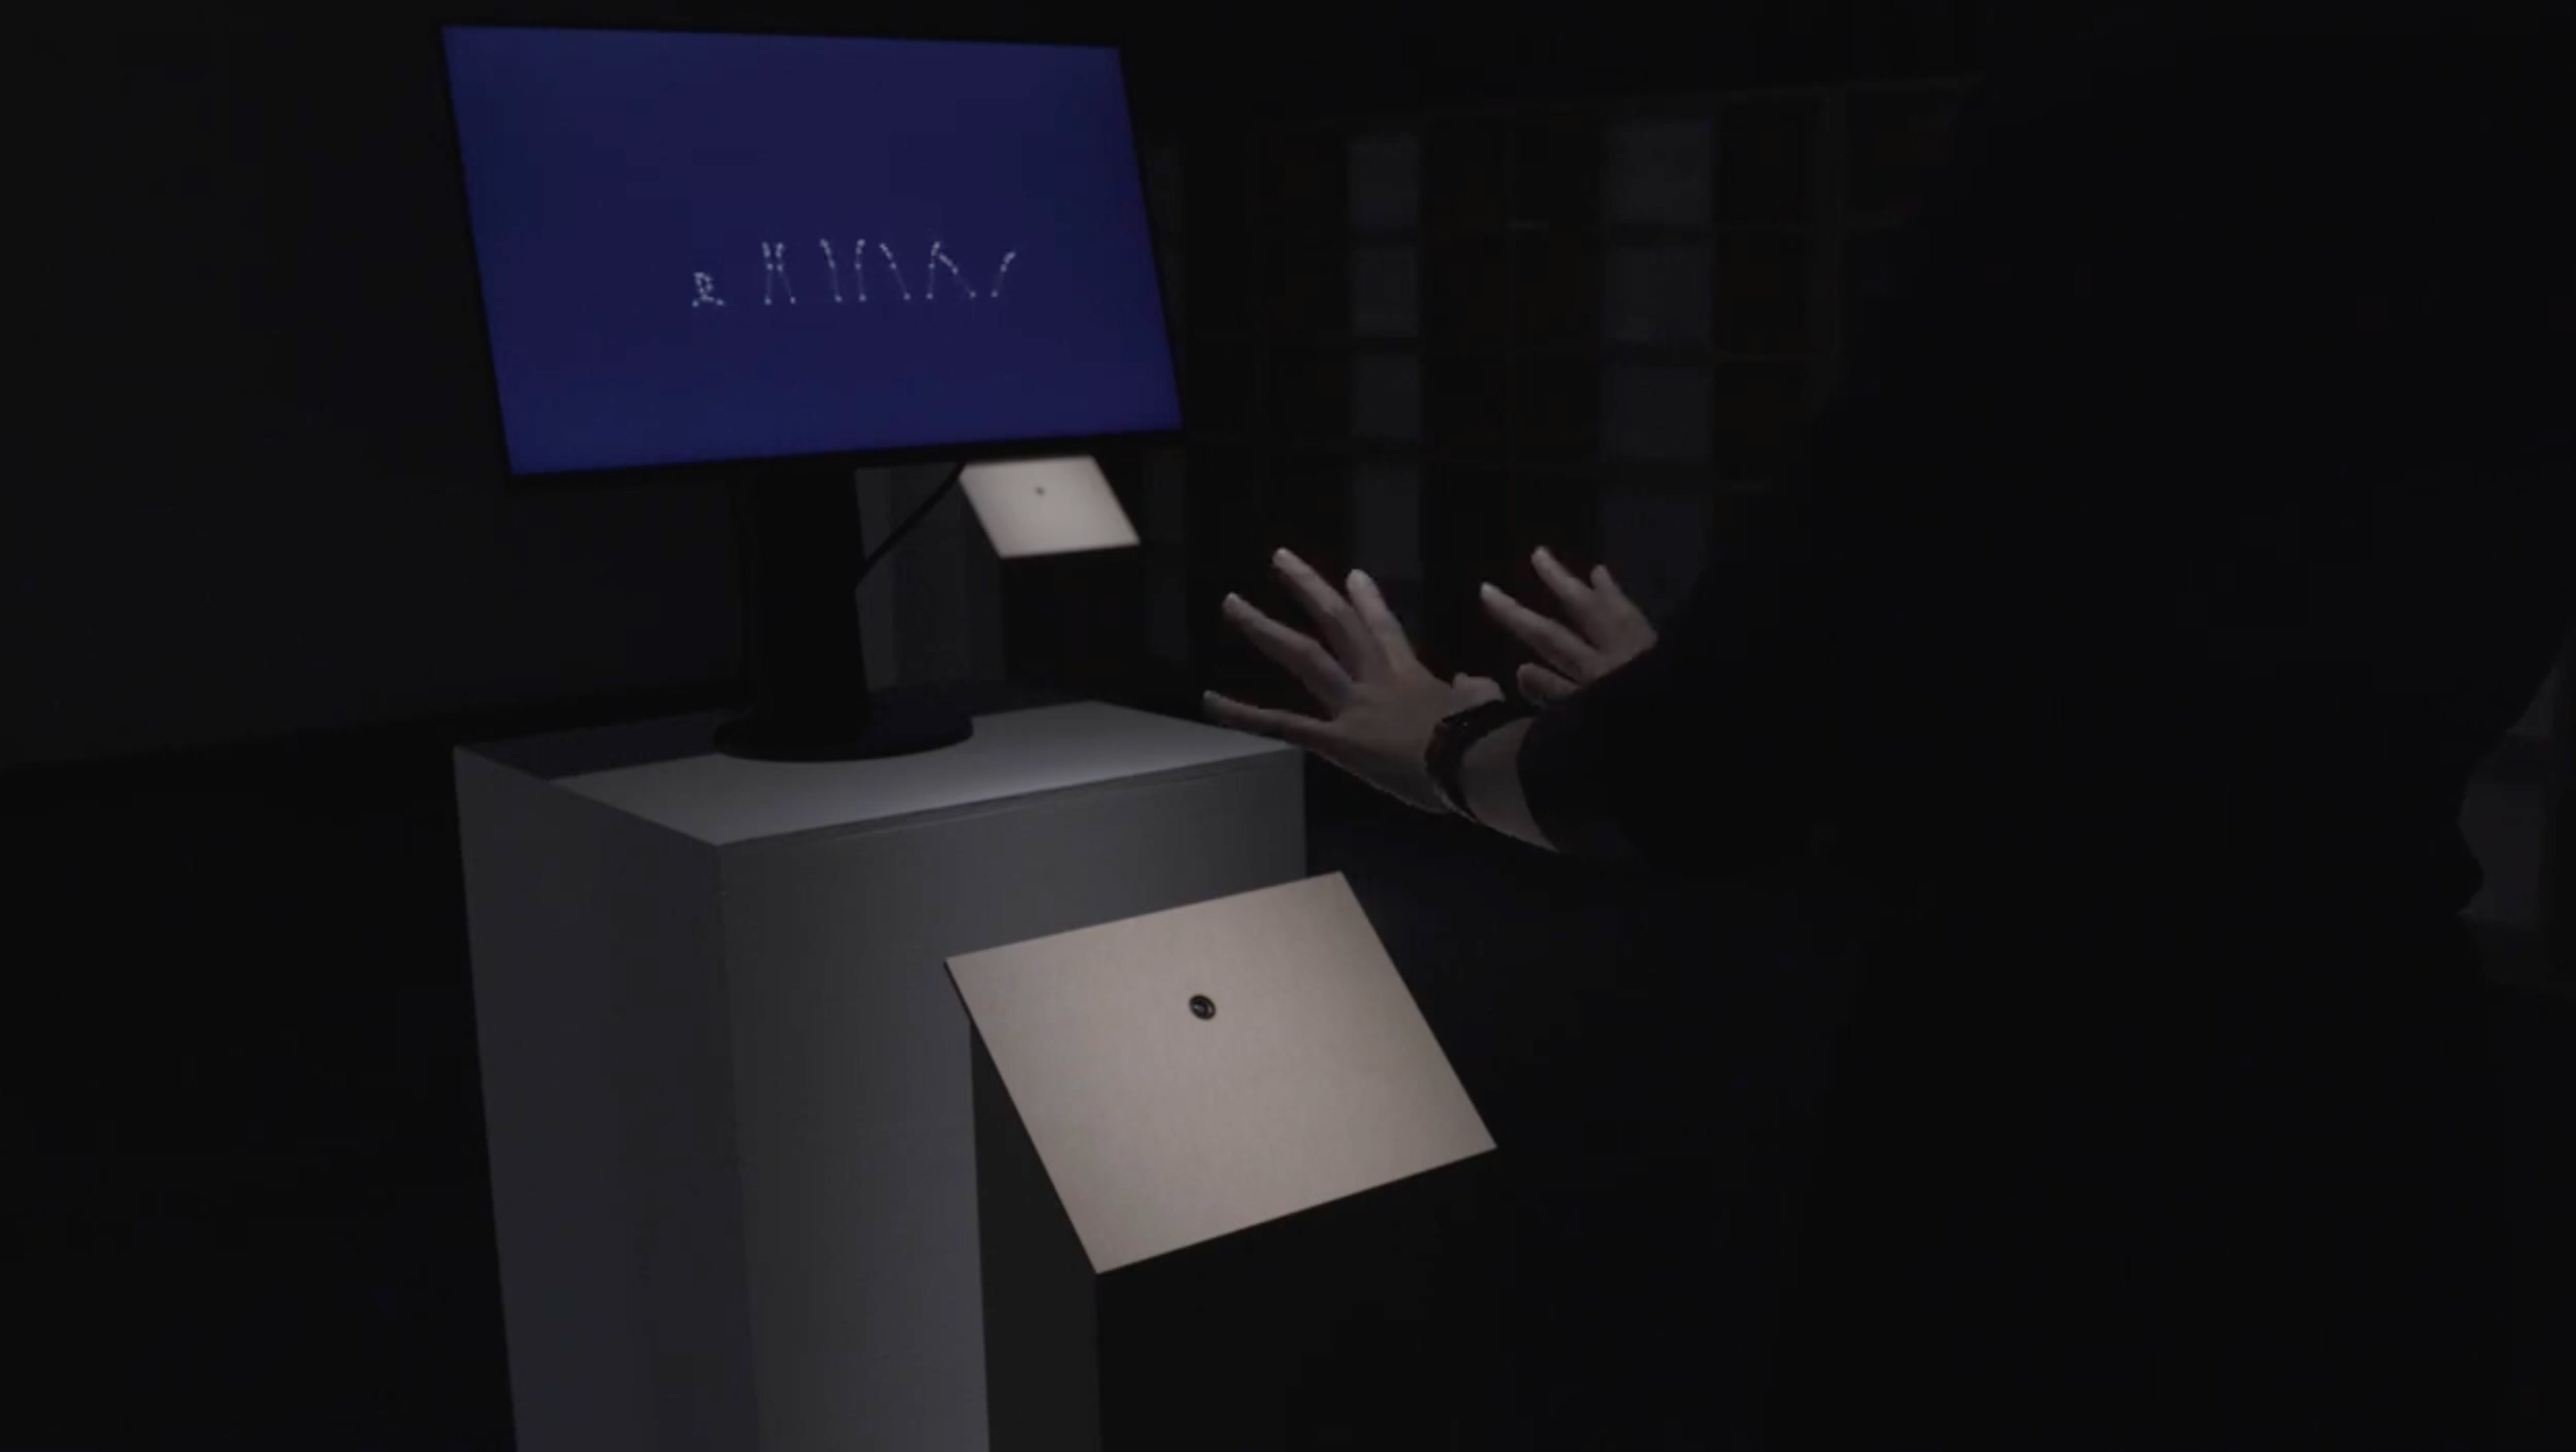
\includegraphics[width=15cm]{img/kyotai_ver2.png}
  \caption{作品展示の際の筐体}
  \label{fig:kyotai_ver2}
\end{figure}

筐体の高さは腰ほどの高さ(850mm)とすることで、キーボードのブラインドタッチのように、画面を見ながら手を同時に見ることが難しい構成とした。

カメラは、鉛直上向ではなく斜めを向いているので、筐体の前に立つと体験者の身体と手指の位置が重なり、トラッキングしやすい状況ができる。

また、ライティングの調整によってトラッキングの精度を高めた。
最終的な展示形態では、スポットライトを当てることで筐体周りを明るくすると同時に照り返しで手元の採光をし、周囲の照明を落とすことで明暗差を作ることで、手指の姿勢を認識しやすくなる。

\begin{figure}[H]
  \centering
  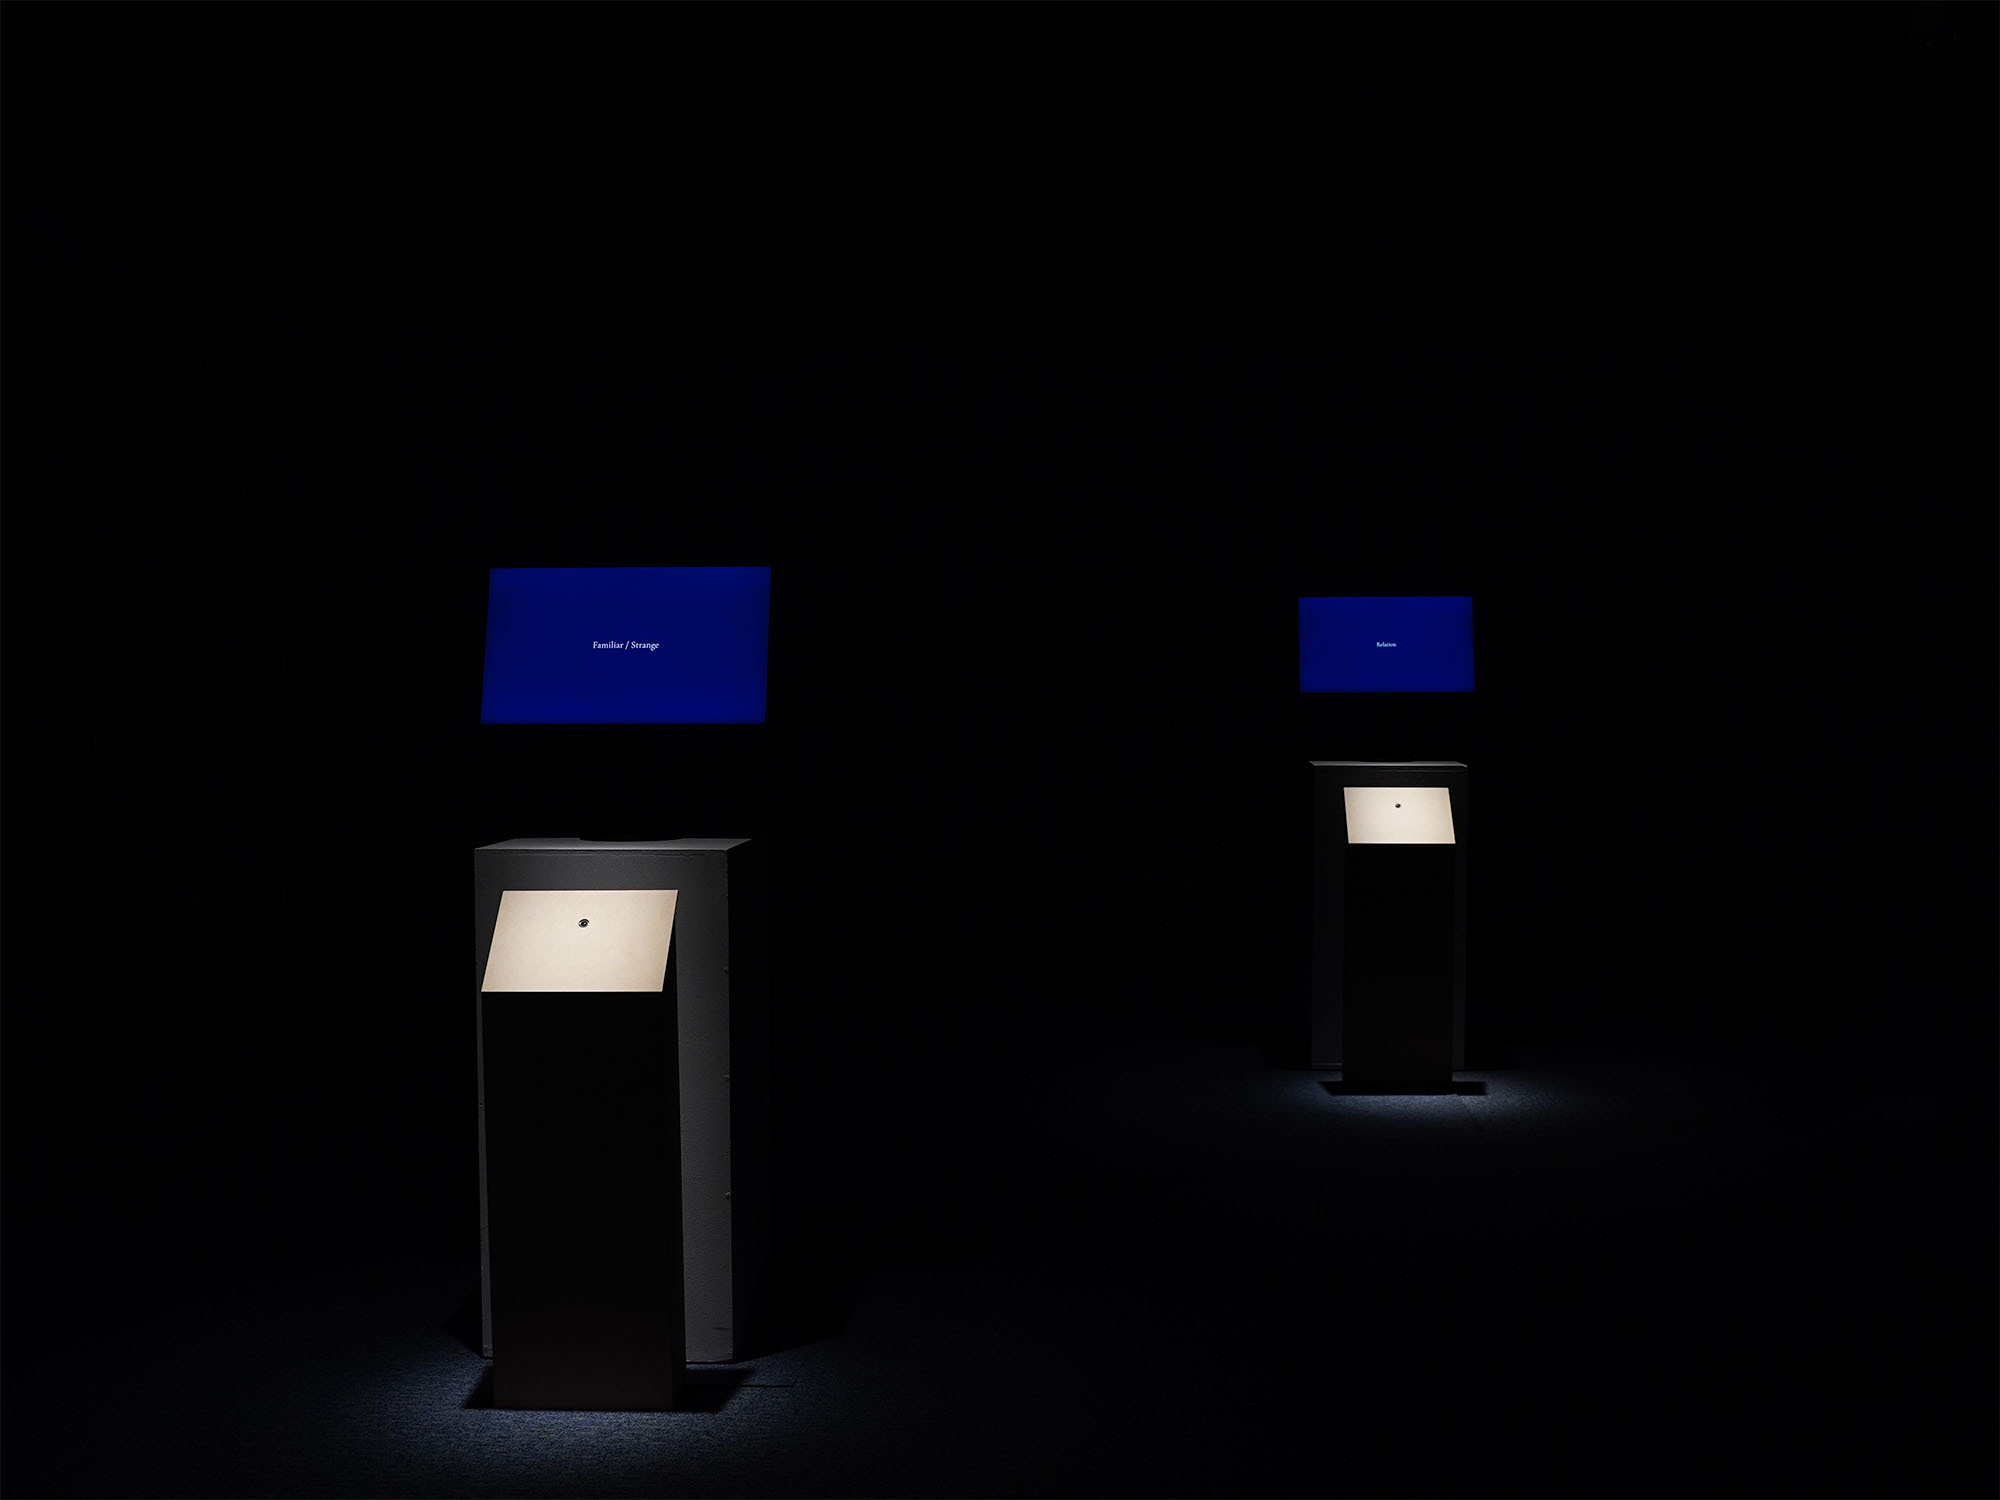
\includegraphics[width=15cm]{img/lighting.jpg}
  \caption{作品展示の際のライティング}
  \label{fig:lighting}
\end{figure}
